\documentclass[conference]{IEEEtran}
\IEEEoverridecommandlockouts

\usepackage{cite}
\usepackage{amsmath,amssymb,amsfonts}
\usepackage{algorithmic}
\usepackage{graphicx}
\usepackage{textcomp}
\usepackage{xcolor}
\usepackage{booktabs}
\usepackage{hyperref}
\usepackage{subcaption}
\usepackage{tikz}
\usetikzlibrary{shapes.geometric, arrows.meta, positioning, fit, backgrounds}

\def\BibTeX{{\rm B\kern-.05em{\sc i\kern-.025em b}\kern-.08em
    T\kern-.1667em\lower.7ex\hbox{E}\kern-.125emX}}

\begin{document}

\title{Message-Passing Graph Neural Network as a Surrogate for Variable-Length 1D Finite Element Bead Chain Simulations}

\author{
\IEEEauthorblockN{Grey L. Goodwin}
\IEEEauthorblockA{\textit{Dept. of Electrical and Computer Engineering} \\
\textit{University of Kentucky}\\
Lexington, KY, USA \\
grey.goodwin@uky.edu}
\and
\IEEEauthorblockN{Daniel L. Lau, PhD.}
\IEEEauthorblockA{\textit{Dept. of Electrical and Computer Engineering} \\
\textit{University of Kentucky}\\
Lexington, KY, USA \\
dllau@uky.edu}
}

\maketitle

\begin{abstract}
Finite element analysis (FEA) of a flexible bead chain requires thousands of small, localized force and integration computations per simulated second. We train a graph neural network (GNN) to predict the per-timestep physics of a 1D bead chain with tapered mass, using randomly sampled single-step training data instead of recorded simulations. A key finding was that even a well-designed model will fail without the correct training data. Sampling neighbor positions in polar coordinates near the rest length was necessary for stable rollouts, while uniform Cartesian sampling produced models that diverged. With this data pipeline in place, an initial multilayer perceptron (MLP) achieved accurate predictions on a fixed 16-bead chain but would require further training for a chain of a different length. We address this by restructuring the network as a true message-passing GNN with separate encoders for node and edge features, ghost masking for chain endpoints, and weight sharing across all nodes. The same trained model runs on chains of any length. We train on 1M per-bead samples drawn from chains of 8 to 32 beads with random taper ratios. Once trained, we were able to evaluate rollout accuracy, constraint satisfaction, and generalization on chain lengths never seen during training. The model maintains accurate performance across the trained range and handles varied initial orientations and velocities. We discuss the connection between the local message-passing structure and the underlying physics, the relationship between sampling strategy and generalization, and remaining limitations.
\end{abstract}

\begin{IEEEkeywords}
graph neural network, finite element analysis, message passing, surrogate model, bead chain, volume sampling
\end{IEEEkeywords}

% ==========================================================================
\section{Introduction}
% ==========================================================================

Physical simulations of flexible one-dimensional structures such as whips, ropes, cables, and biological filaments are common in physics simulation and animation. The standard formulation models the structure as a chain of mass nodes connected by rod elements~\cite{bathe1996finite}, applies local force laws, and integrates forward in time. Even simple cases need small timesteps and many integration steps, so long simulations are expensive even though each step only updates position and velocity by an increment of $\Delta t = 10^{-4}$~s.

Machine learning surrogates for physics simulations offer a way to speed this up. Graph neural networks (GNNs) are a natural fit for mesh-based simulations because the mesh itself is a graph. Nodes are the mesh points, edges are elements, and the local physics at each node depends only on its immediate neighbors. A trained GNN that respects this graph structure can replace the per-timestep numerical computation with a single forward pass. Battaglia et al.~\cite{battaglia2016interaction} introduced the interaction network formulation that underlies many modern physics GNNs. Sanchez-Gonzalez et al.~\cite{sanchez2020learning} demonstrated GNN surrogates for particle systems, Pfaff et al.~\cite{pfaff2020learning} extended this to dynamic meshes, and Shivaditya et al.~\cite{shivaditya2022gnn} applied GNN surrogates to finite element meshes.

This paper explores that idea on a 1D FEA bead chain that models a whip. The chain has $N$ mass nodes connected by $N-1$ spring rod elements, with a tapered mass distribution from a heavy fixed anchor to a light free tip. Each bead's next state depends only on its own state and the states of its immediate neighbors, a property we refer to as locality. The reference solver uses symplectic Euler integration~\cite{hairer2006geometric}.

A critical finding during this work was that the training data pipeline matters as much as the model architecture. Uniform Cartesian sampling for neighbor positions produced models that diverged during rollout, while polar coordinate sampling near the rest length produced stable, accurate predictions (Section~II-C).

The MLP surrogate was limited to a fixed 16-bead chain (Section~II-D). We restructure the surrogate as a true message-passing GNN~\cite{gilmer2017neural} with separate node and edge encoders, message functions applied per edge, and ghost masking for chain endpoints. Because all learned functions have shared weights applied per node, the same trained model handles chains of any length. We train on per-bead samples drawn from chains of varying lengths and taper ratios, and we verify that the model generalizes to chain lengths not seen during training. Previous work within our research group on the MeltFlow compressible Euler problem demonstrated that simple concatenation works for 1D fixed-topology meshes, informing the architectural comparison in Section~V-A.

The contributions of this paper are:
\begin{enumerate}
    \item Polar coordinate sampling near the rest length is necessary for stable rollouts. Uniform Cartesian sampling produces models that diverge.
    \item A variable-length message-passing GNN architecture for 1D bead chain physics, compatible with per-bead volume-sampled training data.
    \item A data generation procedure that samples single-step physics scenarios uniformly across chain lengths, taper ratios, and local states, enabling training without trajectory rollouts.
    \item An empirical evaluation of the resulting surrogate on chain lengths, initial orientations, and initial velocities that were not seen during training.
\end{enumerate}

% ==========================================================================
\section{Background and Problem Formulation}
% ==========================================================================

This section describes the physical system, its natural graph structure, and two findings that preceded the main architectural contribution: the importance of sampling strategy and the limitations of the initial MLP surrogate.

\subsection{Bead Chain Physics}

The chain consists of $N$ mass nodes connected by $N-1$ rod elements. Node 0 is fixed at an anchor point; nodes $1, \ldots, N-1$ are free. Each bead has mass $m_i$, position $\mathbf{x}_i \in \mathbb{R}^2$, and velocity $\mathbf{v}_i \in \mathbb{R}^2$. Mass is distributed with a linear taper controlled by a ratio $r = m_0 / m_{N-1}$. A ratio of $r = 10$ produces a whip-like gradient from heavy anchor to light tip.

Three forces act on each free bead: gravity, rod spring forces from each connected neighbor (Hooke's law), and optional viscous damping along the rod axis. A small global velocity drag damps overall motion.

For rod element $e$ connecting beads $i$ and $j$ with rest length $\ell_0$, the spring force is
\begin{equation}
    \mathbf{F}_{ij}^{\text{spring}} = k \, (d - \ell_0) \, \hat{\boldsymbol{\delta}},
    \label{eq:spring}
\end{equation}
where $d = |\mathbf{x}_j - \mathbf{x}_i|$, $\hat{\boldsymbol{\delta}} = (\mathbf{x}_j - \mathbf{x}_i)/d$, and $k$ is the spring stiffness. A viscous damping force $\mathbf{F}_{ij}^{\text{damp}} = c \, ((\mathbf{v}_j - \mathbf{v}_i) \cdot \hat{\boldsymbol{\delta}}) \, \hat{\boldsymbol{\delta}}$ resists relative motion along the rod axis. Total force on bead $i$ is the sum of gravity, drag, and contributions from left and right rods.

Time integration uses symplectic (semi-implicit) Euler:
\begin{align}
    \mathbf{v}_i^{n+1} &= \mathbf{v}_i^n + \Delta t \, \mathbf{a}(\mathbf{x}^n) \label{eq:symp_v}\\
    \mathbf{x}_i^{n+1} &= \mathbf{x}_i^n + \Delta t \, \mathbf{v}_i^{n+1} \label{eq:symp_x}
\end{align}
The position update uses the new velocity $\mathbf{v}_i^{n+1}$, not the old one. This prevents energy from drifting over long simulations.

For the experiments in this paper we use $k = 10^4$ N/m, $c = 0.5$, $\Delta t = 10^{-4}$ s, $N = 16$ unless otherwise stated, total chain length $L = 2.0$ m, total mass $M = 0.5$ kg, and taper ratio $r = 10$.

\subsection{Graph Structure of the Problem}

The finite element mesh is naturally a graph. Nodes are beads with features $(\mathbf{v}, m, \text{is\_fixed})$; edges are rods with features $(\Delta\mathbf{x}, \Delta\mathbf{v}, m_{\text{nbr}}, \ell_0)$ where the $\Delta$ quantities are relative to the neighbor. Each interior bead has exactly two neighbors (left and right). Endpoint beads (bead 0 and bead $N-1$) have only one neighbor each.

For one timestep, the physical interaction is strictly one hop. The force on bead $i$ depends only on $\mathbf{x}_i$, $\mathbf{v}_i$, $m_i$, and the equivalent quantities for its immediate neighbors $i-1$ and $i+1$. No three-body or longer-range interaction exists. This locality is why each bead only needs information from its direct neighbors.

\subsection{Training Data: Why Sampling Strategy Matters}

Before settling on the message-passing architecture, we found that the training data sampling strategy is crucial. Our initial approach sampled neighbor positions uniformly in Cartesian coordinates within a bounding box. This produced training samples where neighbor distances were often far from the rest length, creating spring forces many times larger than any that occur during actual simulation. The resulting models trained to low loss but diverged immediately during rollout because the force magnitudes they learned did not match the forces they encountered at inference time.

The fix was polar coordinate sampling. For each training sample, the neighbor's relative position is drawn with radius uniformly in $[0.95\,\ell_0,\; 1.05\,\ell_0]$ and angle uniformly in $[0, 2\pi)$. This ensures every training sample has a physically realistic rod length, so the model learns force magnitudes that match what it will see when running the model. With this change, even a simple MLP produced stable, accurate rollouts on a fixed 16-bead chain.

\subsection{Initial MLP Surrogate and Its Limitation}

With polar-sampled training data, our first surrogate was a shared MLP that took a 16-dimensional concatenated feature vector per bead: 4 self features $[v_x, v_y, m, \text{is\_fixed}]$, 6 left-neighbor features $[\Delta x, \Delta y, \Delta v_x, \Delta v_y, m_{\text{nbr}}, \ell_0]$, and 6 right-neighbor features with the same structure. The output was the four-dimensional change in state $[\Delta x, \Delta y, \Delta v_x, \Delta v_y]$ to be added to the bead's current state.

This architecture is applied per bead with shared weights, so it is sometimes informally called a GNN. However, the model has no separation between node and edge features, no explicit message computation, and no mechanism for handling a varying number of neighbors. The MLP was trained on mass values and rest lengths specific to a 16-bead chain. Running it on a chain of different length would require regenerating training data and retraining the model from scratch.

% ==========================================================================
\section{Method}
% ==========================================================================

We describe the BeadMPGNN architecture that replaces the fixed-size MLP, the volume sampling procedure used to generate training data, and the training setup.

\subsection{Message-Passing GNN Architecture}

We replace the flat MLP with a message-passing GNN (BeadMPGNN). The architecture consists of five learned components:

\begin{itemize}
    \item \textbf{Node encoder}: a residual MLP that maps the four-dimensional node feature vector to a 64-dimensional hidden state.
    \item \textbf{Edge encoder}: a separate residual MLP that maps the six-dimensional edge feature vector (relative to the neighbor) to a 64-dimensional hidden state. The same encoder is used for both left and right edges.
    \item \textbf{Message MLP}: maps an encoded edge to a 64-dimensional message.
    \item \textbf{Node update MLP}: maps the concatenation $[\mathbf{h}_{\text{self}} \| \mathbf{m}_{\text{left}} \| \mathbf{m}_{\text{right}}] \in \mathbb{R}^{192}$ back to a 64-dimensional updated node state.
    \item \textbf{Output head}: a linear layer that projects the final hidden state to the four-dimensional change in state.
\end{itemize}

Fig.~\ref{fig:arch_mlp} and Fig.~\ref{fig:arch_mpgnn} compare the two architectures.

\begin{figure}[t]
    \centering
    \begin{subfigure}[t]{\columnwidth}
        \centering
        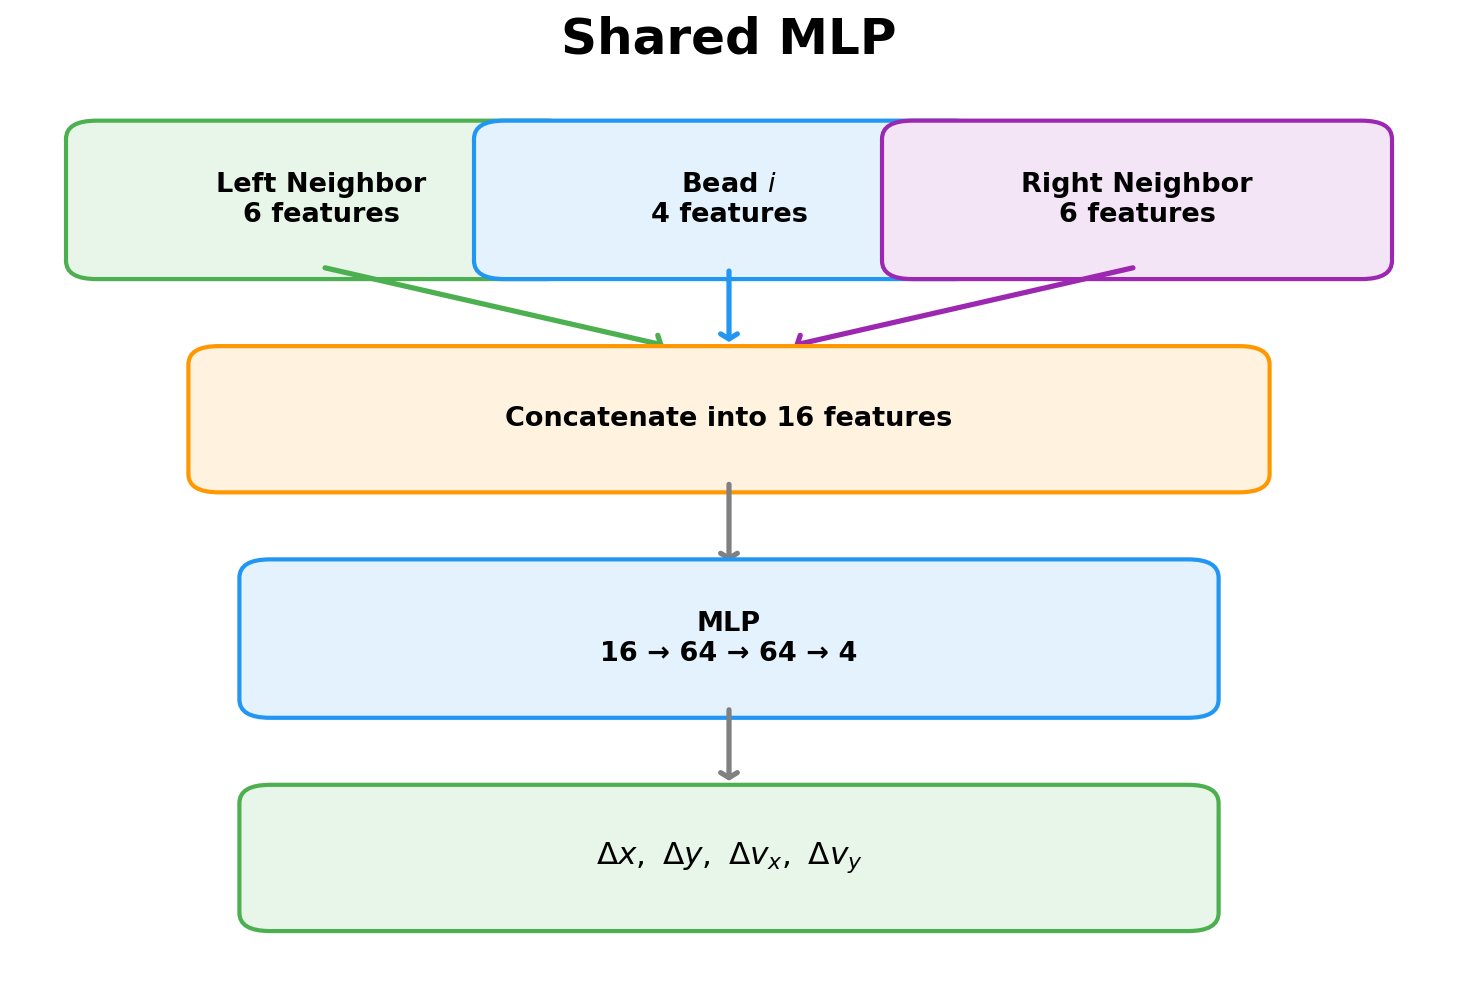
\includegraphics[width=\columnwidth]{architecture_mlp_only.png}
        \caption{The shared MLP concatenates all 16 features into a single vector.}
        \label{fig:arch_mlp}
    \end{subfigure}
    \begin{subfigure}[t]{\columnwidth}
        \centering
        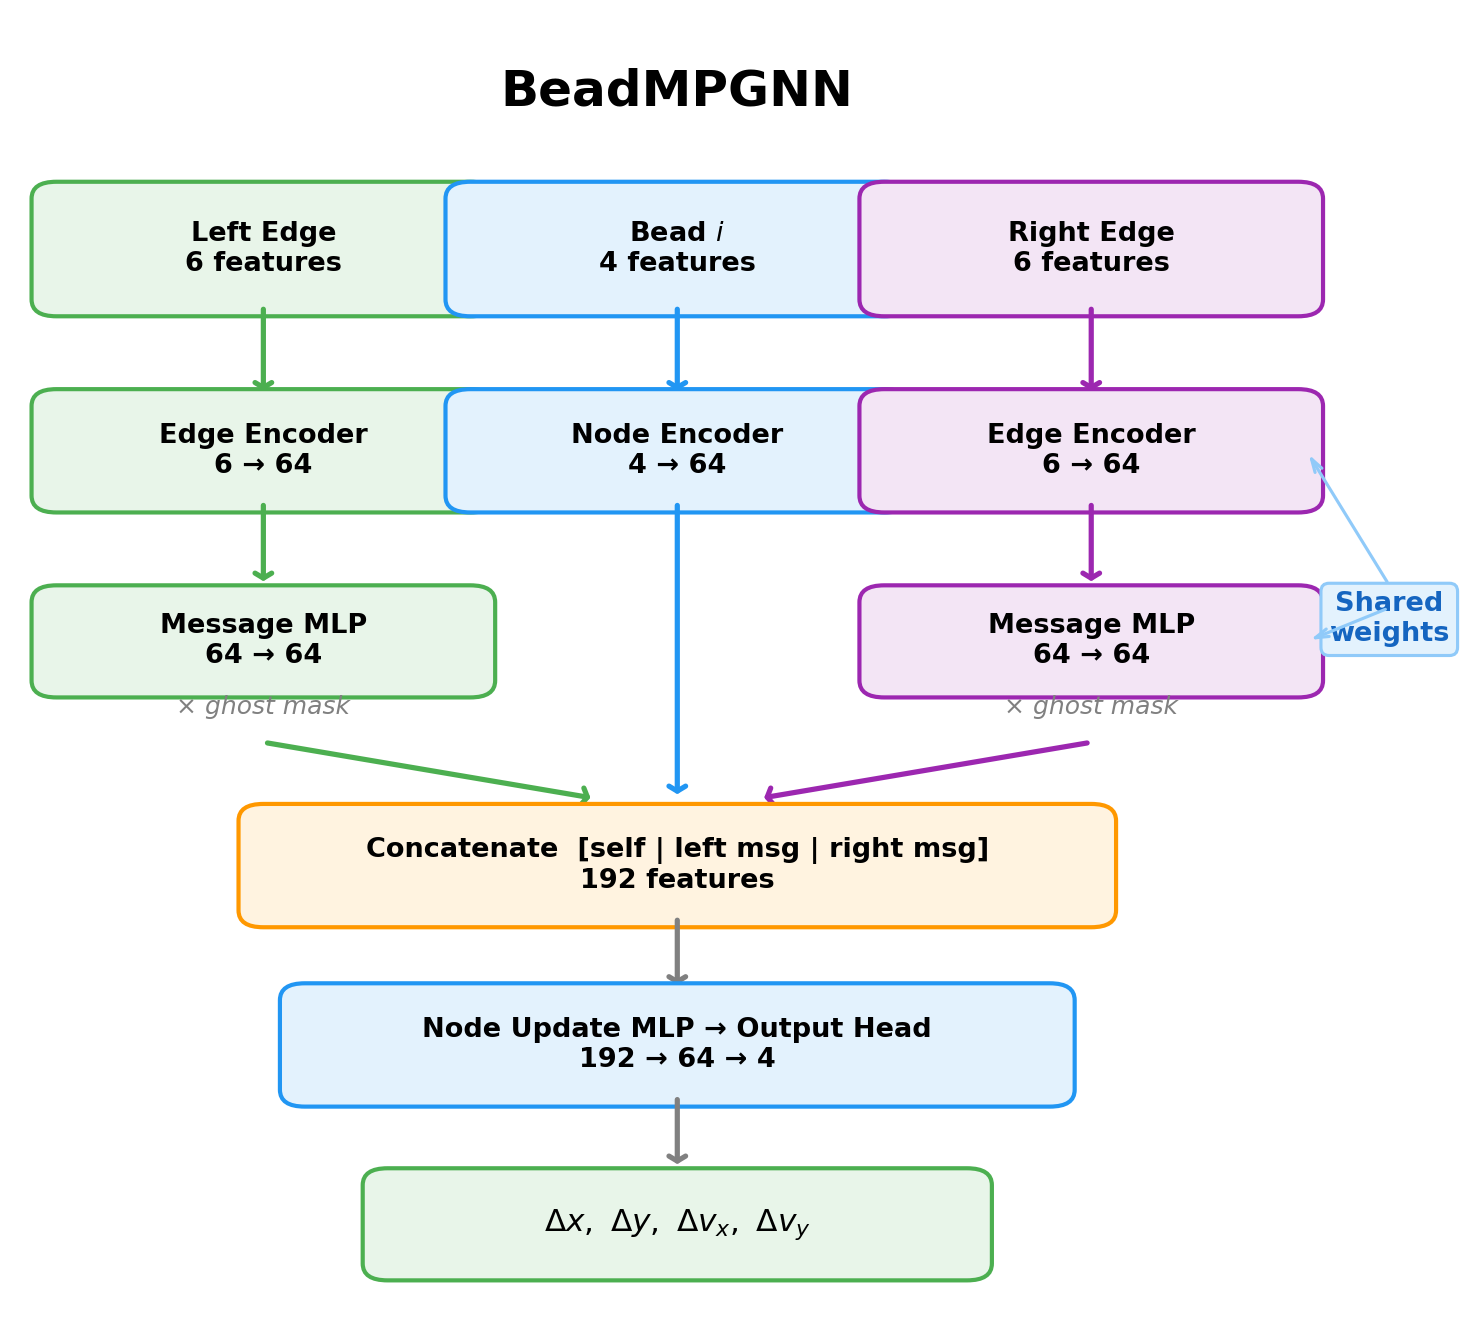
\includegraphics[width=\columnwidth]{architecture_mpgnn_only.png}
        \caption{The BeadMPGNN encodes node and edge features separately, computes messages per edge, applies ghost masking for missing neighbors, and concatenates the results before the node update.}
        \label{fig:arch_mpgnn}
    \end{subfigure}
    \caption{Architecture comparison. (a) Shared MLP. (b) BeadMPGNN.}
    \label{fig:architecture}
\end{figure}

Each bead's forward pass proceeds as follows:
\begin{enumerate}
    \item Normalize input features using stored per-feature mean and standard deviation, computed once from the training set and fixed during training.
    \item Encode self state and both edges through their respective encoders.
    \item Compute left and right messages by passing each edge encoding through the message MLP.
    \item Zero out messages from absent neighbors via ghost masking: $\mathbf{m}_L \leftarrow \mathbb{1}_{\text{has\_left}} \cdot \mathbf{m}_L$, and similarly for right.
    \item Concatenate $[\mathbf{h}_{\text{self}} \| \mathbf{m}_L \| \mathbf{m}_R]$ and run through the node update MLP.
    \item Apply the output head and denormalize to obtain the change in state $[\Delta x, \Delta y, \Delta v_x, \Delta v_y]$.
    \item Add the deltas to the current state to produce the next state.
\end{enumerate}

The total parameter count is 80{,}324. All weights are shared across all beads in a chain, regardless of chain length.

Two architectural choices enable variable-length operation. First, ghost masking ensures that absent neighbors contribute nothing. When bead 0 processes its left edge features (which are zero because no left neighbor exists), the edge encoder and message MLP produce some nonzero output. This output is multiplied by the zero mask, forcing it to zero before the node update. Second, all learned functions are weight-shared and applied per bead. A 32-bead chain uses the same 80K parameters as an 8-bead chain; only the number of per-bead forward passes changes.

For this paper we use one round of message passing ($K=1$), which matches the physics since each bead only interacts with its direct neighbors. Deeper architectures are possible but would require multi-hop training data or end-to-end rollout training to be effective.

\subsection{Volume-Sampled Per-Bead Training Data}

Rather than generating training data by recording simulation trajectories, we sample single-step physics scenarios uniformly across the reachable state space. Each training sample represents one bead at one instant plus the exact physics result for its state one timestep later. No simulation is ever run during data generation. Each sample is a completely independent random scenario solved by direct evaluation of the physics equations.

The procedure for one sample is:
\begin{enumerate}
    \item Draw a chain length $N \sim \text{Uniform}(8, 32)$ and a taper ratio $r \sim \text{Uniform}(1, 10)$.
    \item Compute the tapered mass distribution for that chain and pick a random bead index $i \in \{0, \ldots, N-1\}$.
    \item Draw self velocity $(v_x, v_y)$ uniformly from empirically observed trajectory bounds.
    \item Draw each neighbor's relative position in polar coordinates: radius near the rest length $\ell_0$ (within $\pm 5\%$) and angle uniformly in $[0, 2\pi)$. Draw relative velocities uniformly from observed bounds.
    \item If the bead has no left or no right neighbor, the corresponding features are set to zero.
    \item Compute the exact single-step physics (springs, damping, gravity, drag, symplectic Euler) to produce the target state delta.
\end{enumerate}

The output is a dataset of 1{,}000{,}000 samples, each consisting of node features (four dimensions), left-edge features (six dimensions), right-edge features (six dimensions), binary flags for neighbor presence, and four-dimensional target deltas. Fig.~\ref{fig:pipeline} summarizes the pipeline visually.

\begin{figure*}[t]
    \centering
    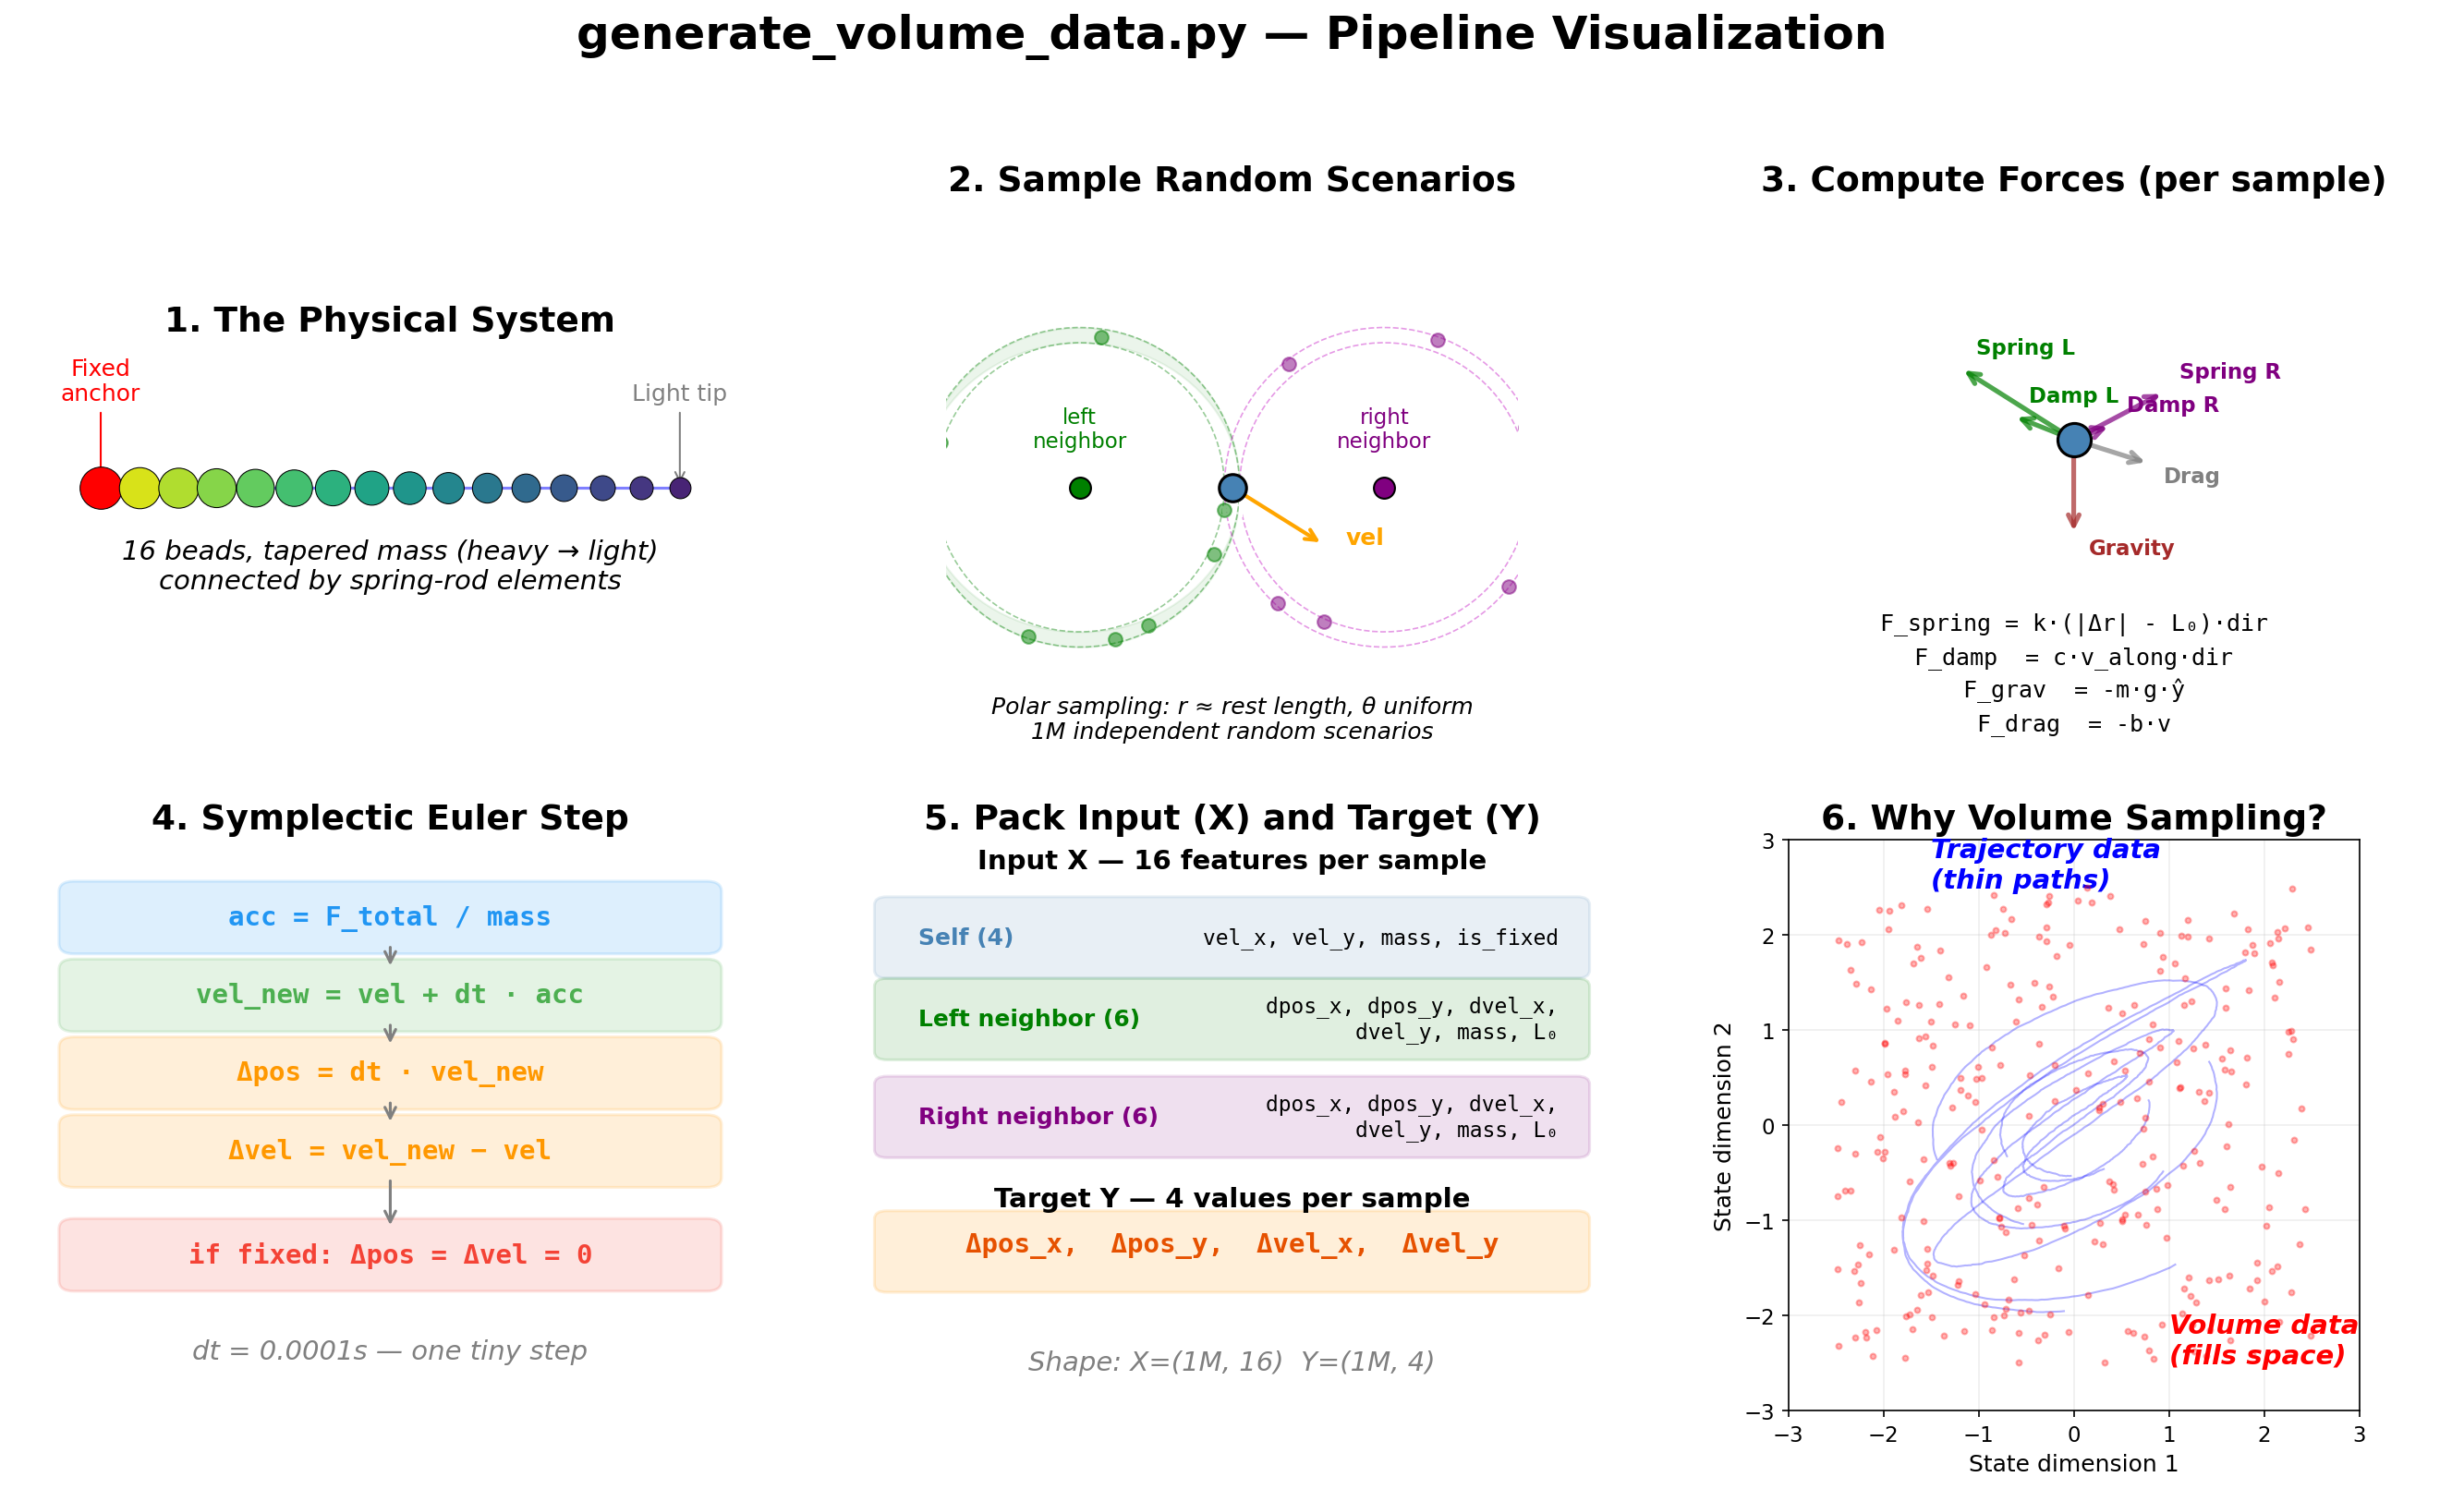
\includegraphics[width=0.95\textwidth]{pipeline_visualization.png}
    \caption{Volume sampling pipeline for generating per-bead training data. (1) The physical system is a tapered chain of 16 beads connected by spring rod elements. (2) Each sample is a random scenario: one bead with left and right neighbors sampled in polar coordinates around rest length. (3) Forces on the central bead are computed analytically. (4) Symplectic Euler advances velocity then position. (5) Input and target arrays are packed. (6) Volume sampling fills the reachable state space uniformly, unlike trajectory data which traces thin paths.}
    \label{fig:pipeline}
\end{figure*}

This sampling strategy covers the reachable state space more uniformly than trajectory recording. A trajectory-based dataset only covers a narrow path through state space. During rollout, small prediction errors push the simulation off this path, where the model has no training coverage and predictions get worse. Volume sampling gives the model training coverage across the full state space, not just along specific trajectories.

\subsection{Training}

We normalize node features and edge features separately, each with its own mean and standard deviation vector computed over the full training set. Targets are normalized the same way. The model trains with mean squared error loss on the normalized deltas.

We use AdamW with weight decay $10^{-5}$ and a cosine annealing learning rate schedule from $10^{-3}$. Batch size is 512 and we train for 200 epochs. A 10\% split is reserved for validation. Gradient clipping at norm 1.0 is applied throughout. The normalization statistics are stored as buffers on the trained model so that inference is fully self-contained.

% ==========================================================================
\section{Results}
% ==========================================================================

We evaluate the trained BeadMPGNN on side-by-side rollouts against the reference solver, training convergence, generalization to unseen chain lengths, and robustness to different initial conditions.

\subsection{Side-by-Side Rollout}

Fig.~\ref{fig:snapshots} shows three snapshots from a side-by-side rollout of the reference solver (left, black) and the BeadMPGNN (right, red) on a 16-bead chain released from horizontal. The bottom panel shows the mean position error over time. The GNN closely tracks the ground truth through the initial fall, the curved swing, and the whip action at the tip. Error grows during the first 0.6 seconds of rapid motion and then plateaus as the chain settles.

\begin{figure}[t]
    \centering
    \begin{subfigure}[t]{\columnwidth}
        \centering
        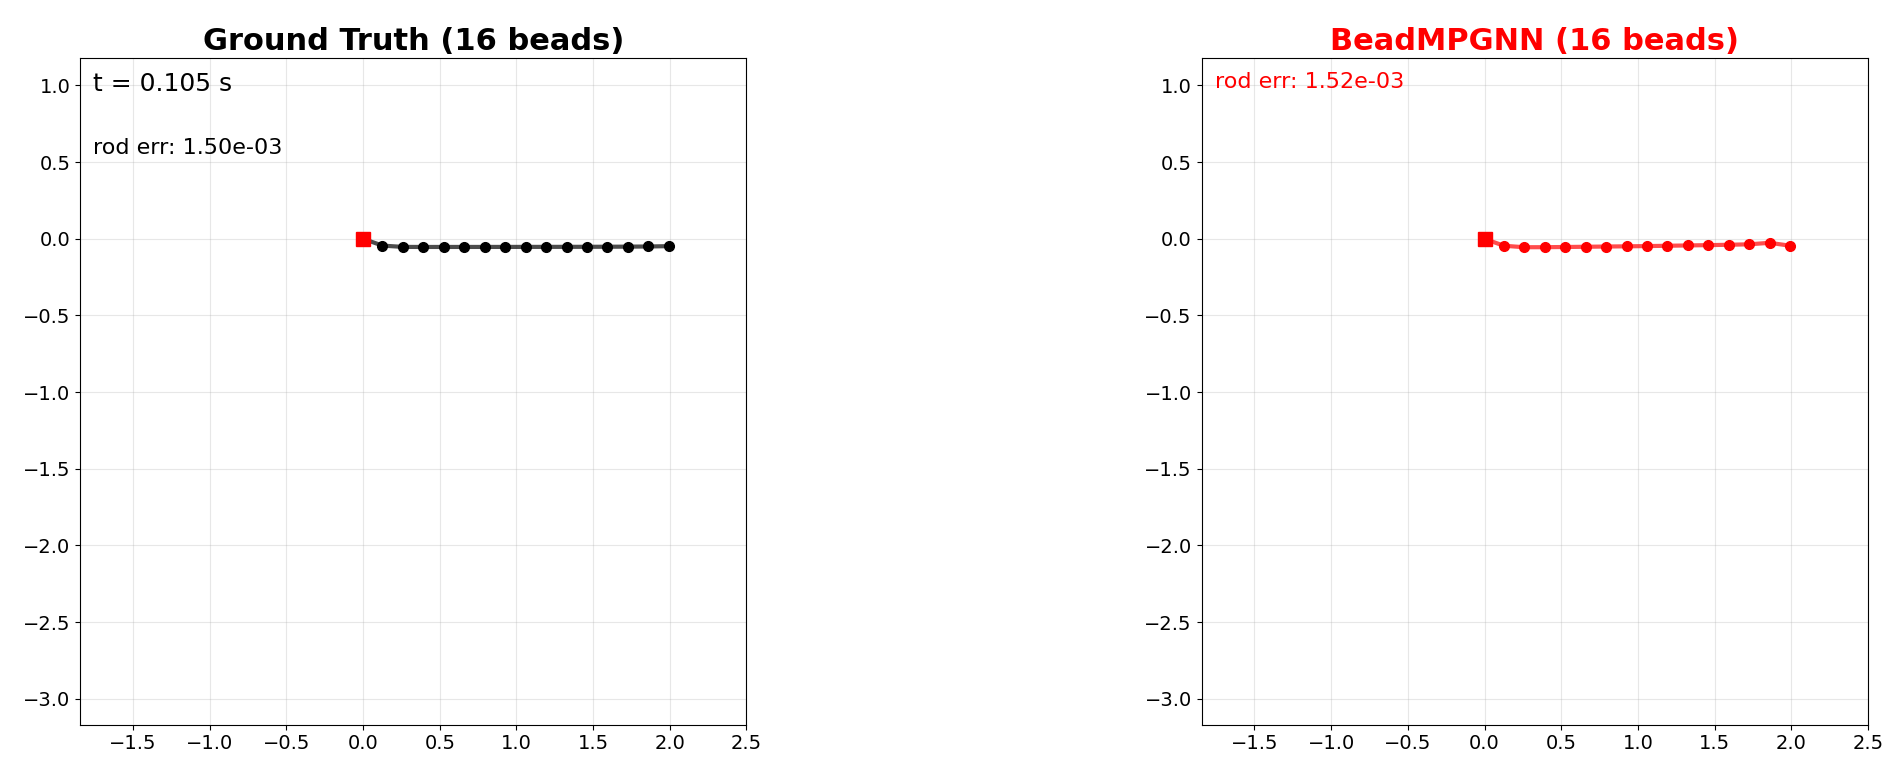
\includegraphics[width=\columnwidth]{frame_initial.png}
        \caption{$t = 0.105$ s. Initial horizontal configuration.}
    \end{subfigure}
    \vskip1ex
    \begin{subfigure}[t]{\columnwidth}
        \centering
        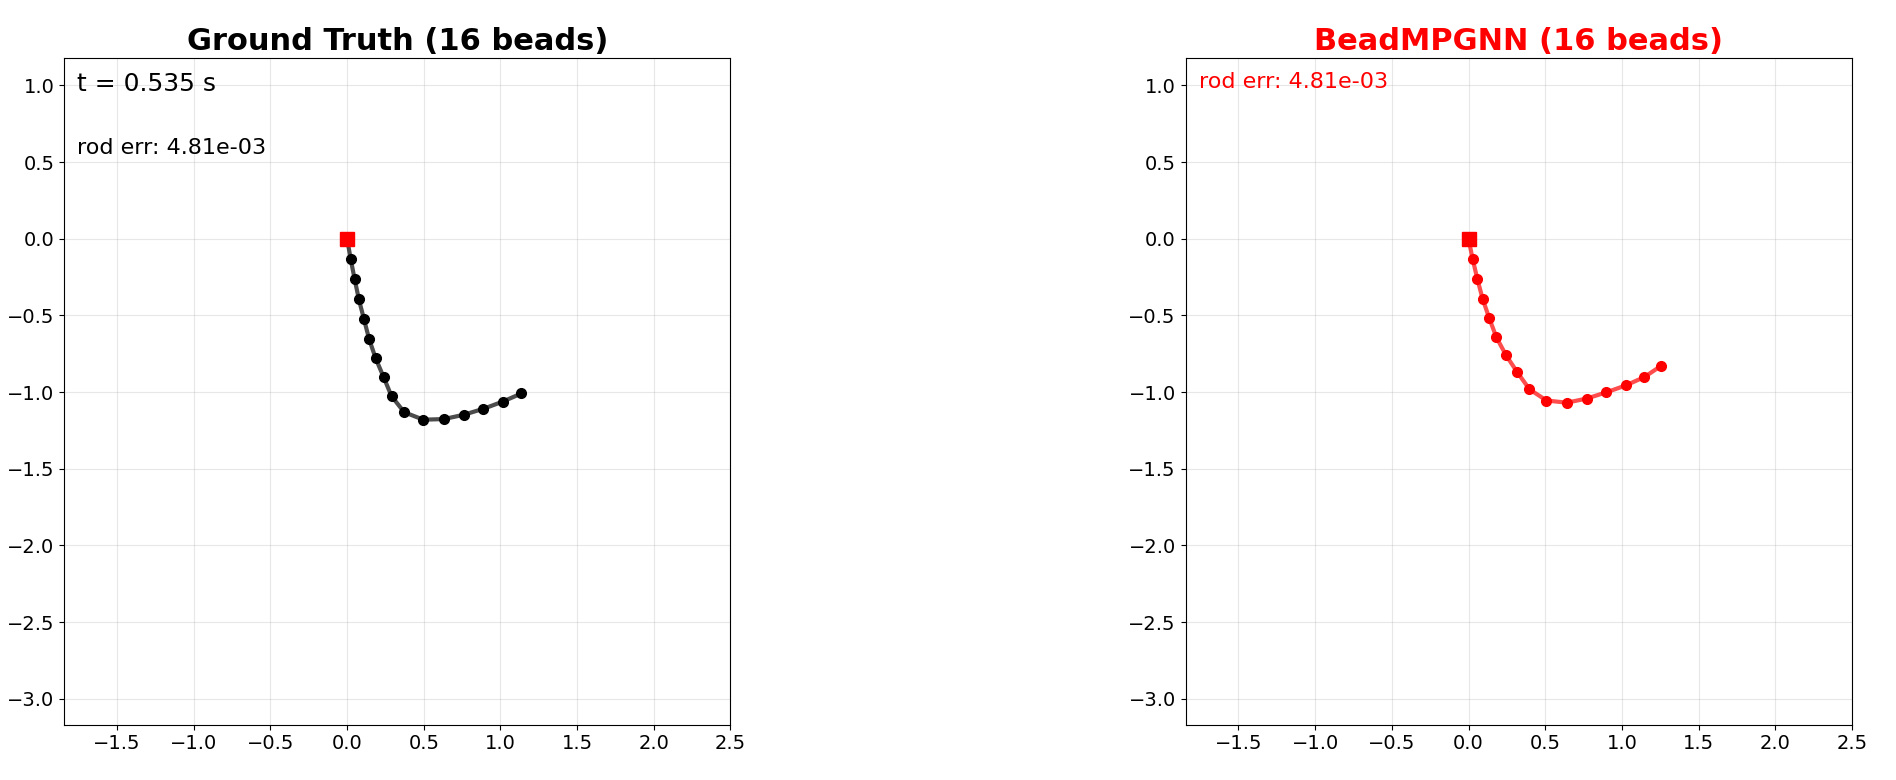
\includegraphics[width=\columnwidth]{frame_falling.png}
        \caption{$t = 0.535$ s. Chain falling under gravity.}
    \end{subfigure}
    \vskip1ex
    \begin{subfigure}[t]{\columnwidth}
        \centering
        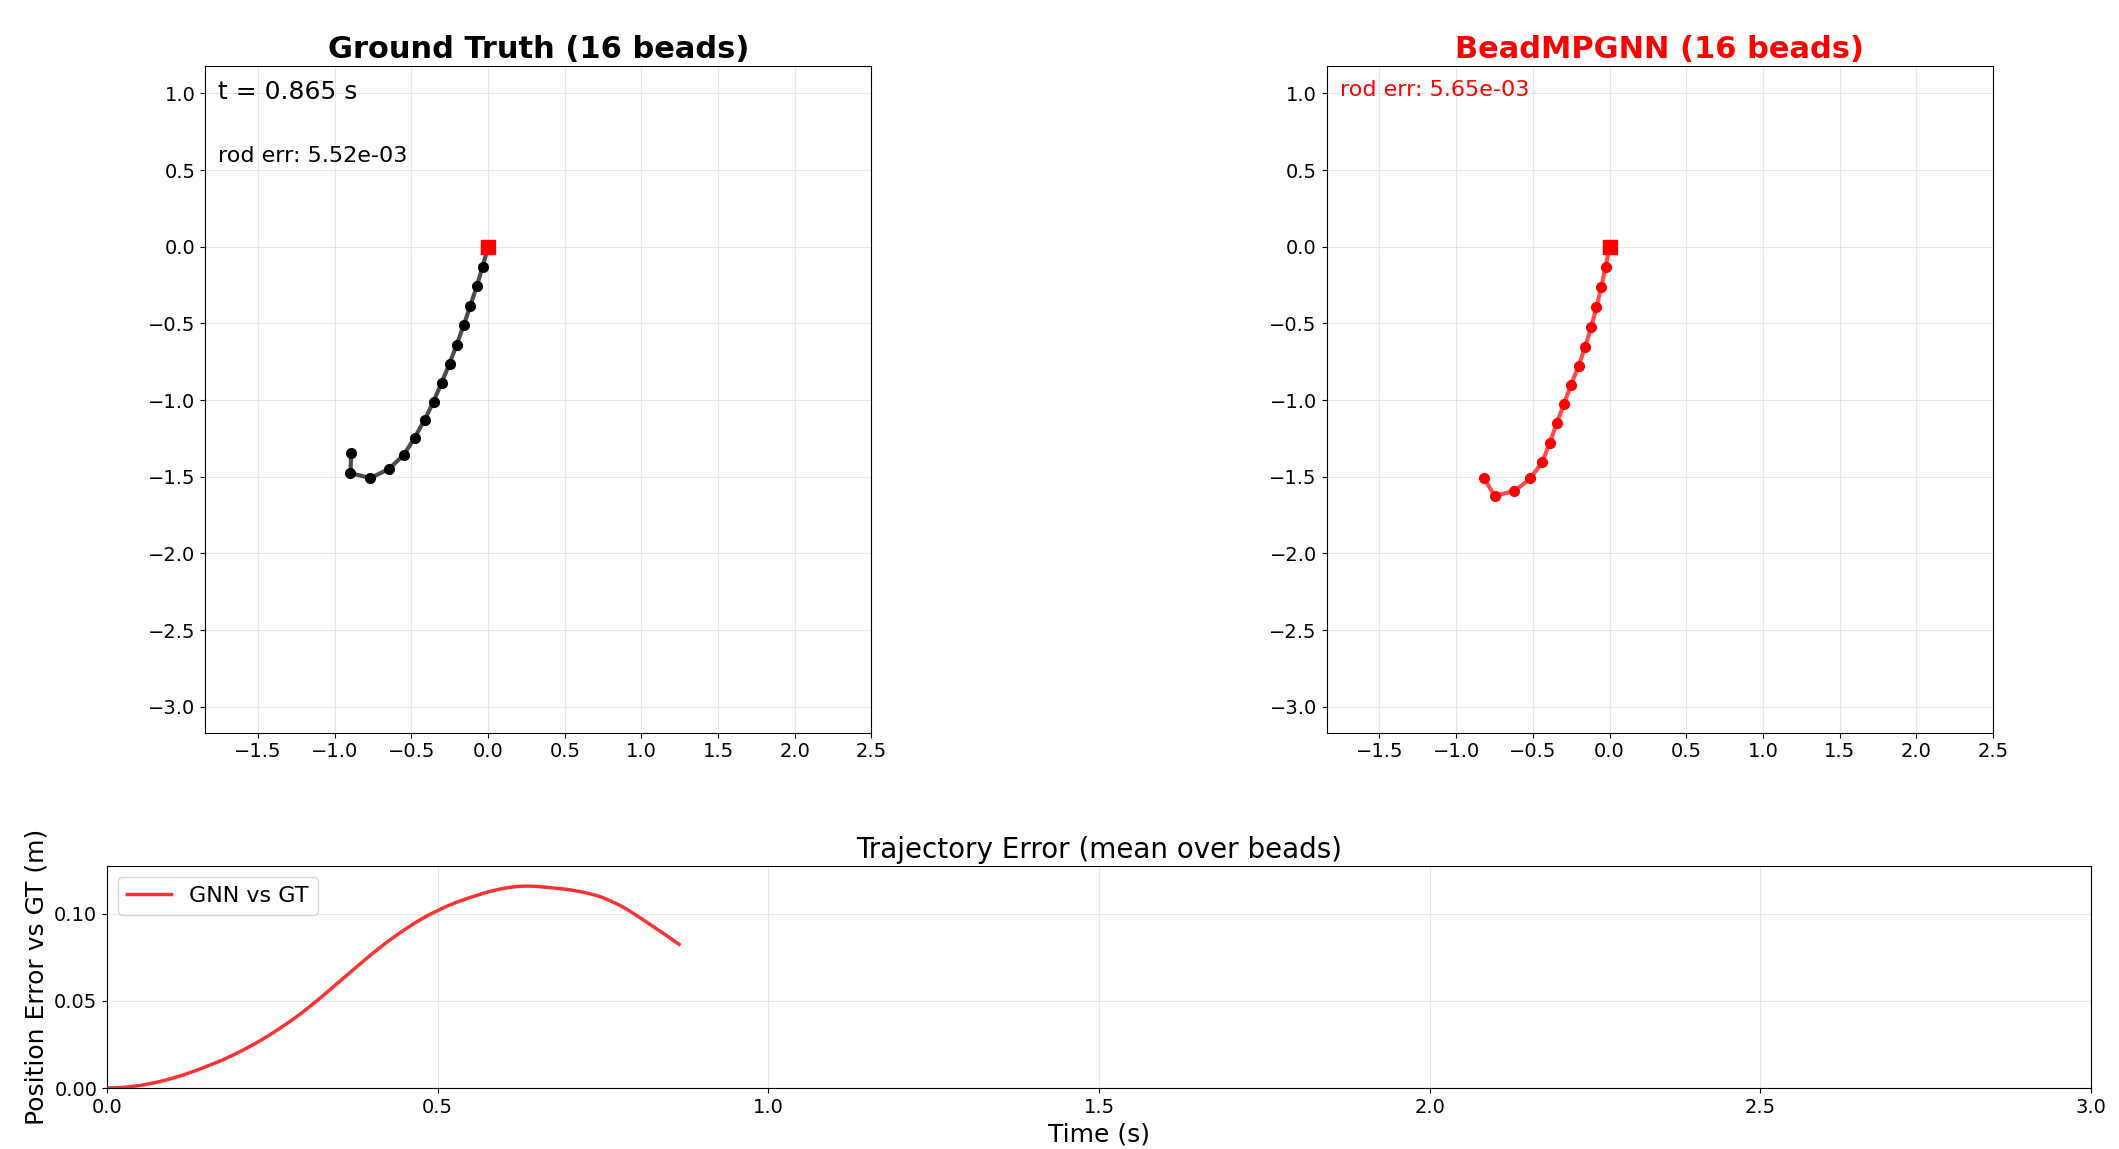
\includegraphics[width=\columnwidth]{frame_whip.png}
        \caption{$t = 0.865$ s. Whip action at the tip. Bottom: mean position error over time.}
    \end{subfigure}
    \caption{Snapshots from a side-by-side rollout of the reference solver (left, black) and BeadMPGNN (right, red) on a 16-bead chain. The bottom panel of (c) shows mean position error over time. The GNN tracks the ground truth through all three phases of motion.}
    \label{fig:snapshots}
\end{figure}

\subsection{Training Convergence}

Training loss decreases smoothly over 200 epochs and tracks the validation loss closely. A scatter of predicted versus true velocity deltas on 200 held-out samples falls tightly along the diagonal, showing that per-sample predictions are accurate. Fig.~\ref{fig:training} shows both plots.

\begin{figure}[t]
    \centering
    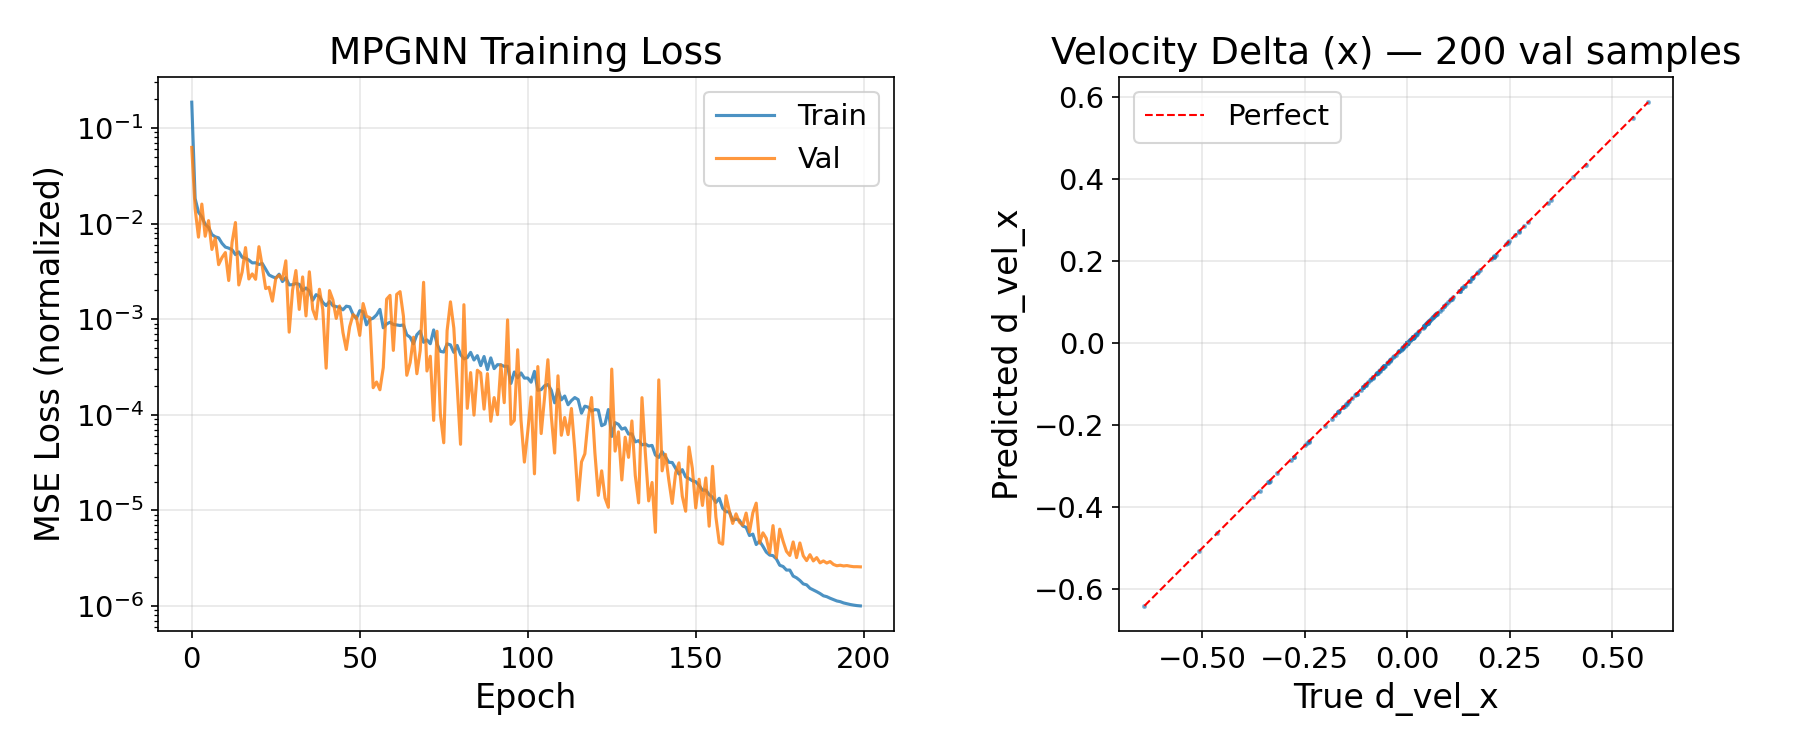
\includegraphics[width=\columnwidth]{mpgnn_training.png}
    \caption{BeadMPGNN training convergence. Left: train and validation MSE loss over 200 epochs on a log scale. Right: predicted versus true velocity delta $\Delta v_x$ on 200 validation samples.}
    \label{fig:training}
\end{figure}

\subsection{Generalization to Unseen Chain Lengths}

The most important test is whether the model trained on chains of 8 to 32 beads can produce accurate rollouts on chain lengths not seen during training. We compare the BeadMPGNN rollout with the reference symplectic Euler solver, starting from identical initial conditions, and measure mean position error across all beads over time.

Fig.~\ref{fig:eval} shows results for chain lengths $N \in \{8, 10, 12, 16, 20, 24, 32\}$. Short to medium chains ($N \le 16$) track the reference closely with low accumulated error. Longer chains ($N \ge 20$) show more drift, consistent with the longer chain having more compounding per-step errors and more numerous light-mass tip beads. Rod length accuracy (maximum relative error) is in the $10^{-3}$ range across all tested lengths, which is acceptable for the stiff-spring formulation.

\begin{figure}[t]
    \centering
    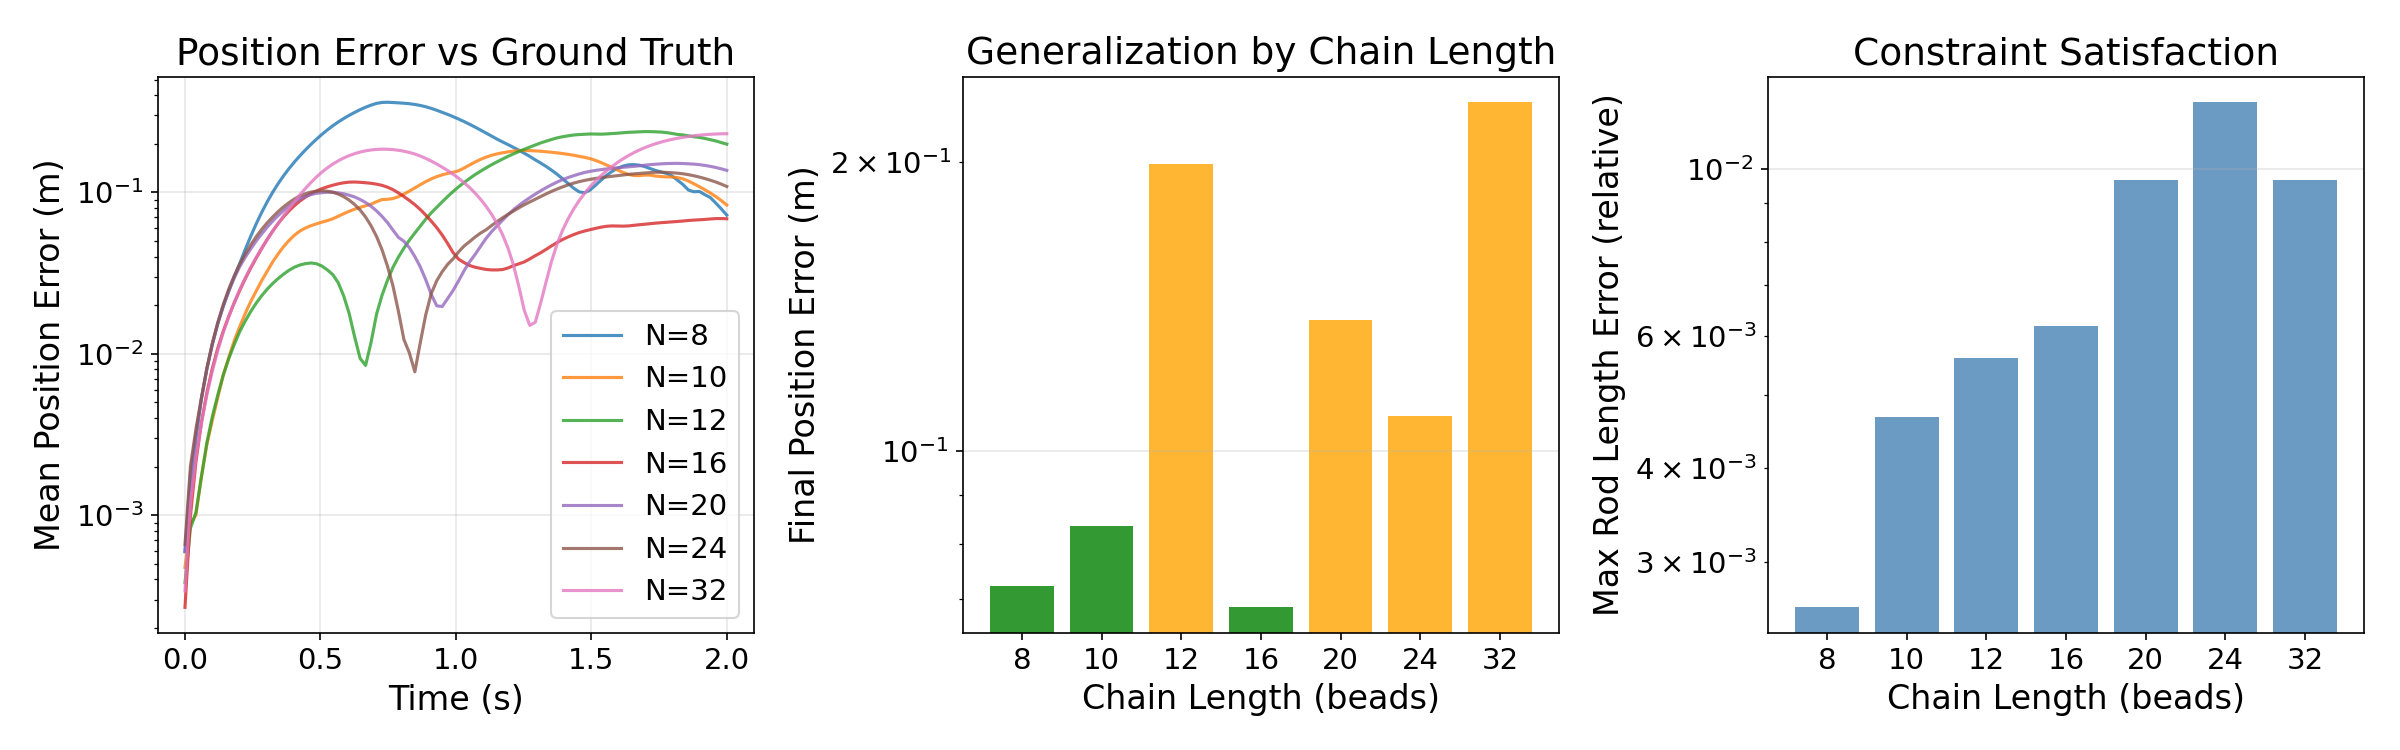
\includegraphics[width=\columnwidth]{mpgnn_variable_eval.png}
    \caption{Generalization across chain lengths. Left: mean position error between MPGNN and reference over 20{,}000 timesteps, by chain length. Center: final position error at $t = 2$ s for each chain length. Right: maximum rod length violation. The model is trained on chains of 8 to 32 beads with random taper ratios, but specific chain lengths such as $N=14$ or $N=18$ are never seen as single-sample configurations during training.}
    \label{fig:eval}
\end{figure}

\subsection{Initial Condition Robustness}

We additionally tested the model under initial conditions outside the typical ``released from horizontal'' default: starting the chain rotated to $45^\circ$ or $90^\circ$ from horizontal, and applying uniform initial velocities (a downward kick of $v_y = -5$ m/s, or a sideways throw of $v_x = 8$ m/s). Because the training data was volume-sampled rather than trajectory-sampled, the model was exposed to many states that correspond to such initial conditions. No specific trajectory from these configurations was recorded. The model handles all tested initial conditions within its training velocity bounds. Pushing velocities significantly outside the sampling bounds (e.g.\ $v_x > 20$ m/s) produces visible divergence, as expected.

% ==========================================================================
\section{Discussion}
% ==========================================================================

We discuss why message passing was necessary for this problem and the current limitations of the approach.

\subsection{Why Message Passing Matters Here}

A prior result within our research showed that for 1D path graphs with fixed topology, the simple concatenation of left and right neighbor states into one MLP input is sufficient to learn local flux functions in compressible fluid problems. The conclusion was that explicit message passing is unnecessary when the graph is a fixed-size path. That conclusion remains valid in its original setting.

Our work addresses a different requirement. The concatenation approach has a fixed input size tied to the chain length. When the goal is a single model that handles multiple chain lengths, the architecture must respect the graph structure explicitly, with separate processing for nodes and edges and shared weights across all beads. The gain is not accuracy per sample. It is the ability to change $N$ when running the model without retraining.

\subsection{Limitations}

\paragraph{Rollout drift} During training, the model always receives the correct state as input. When running the simulation, it receives its own previous prediction instead. If a prediction is slightly off, the next step starts from a slightly wrong state, and the error compounds over thousands of steps. We see this most on long chains where the light tip beads move fast and accumulate error quickly. Training the model on its own outputs (rollout training) would help, but we have not implemented it yet.

\paragraph{Constraint satisfaction} The reference solver uses stiff springs as a soft constraint. We train the GNN to match those spring-based dynamics. The resulting rod length errors are in the $10^{-3}$ range rather than machine zero, which is adequate for visually correct dynamics but not for applications where exact inextensibility matters.

\paragraph{Receptive field} We use $K=1$ rounds of message passing, which matches the locality of one physics timestep. For longer rollouts or more complex graphs, multiple message-passing rounds may be needed. However, training $K>1$ would require training data that captures dependencies beyond direct neighbors. The present volume sampling procedure only covers one step of interaction.

\paragraph{Domain specificity} The model is trained on a specific physical setup (bead chain with gravity, spring rods, damping, drag). Transferring it to a different physical system would require regenerating data and retraining. However, the architecture itself is not problem-specific. Similar patterns apply to any 1D mesh with local interactions.

% ==========================================================================
\section{Conclusion and Future Work}
% ==========================================================================

We have described a variable-length message-passing graph neural network that acts as a per-timestep surrogate for a 1D finite element bead chain. The training data sampling strategy turned out to be as important as the model architecture. Polar coordinate sampling near the rest length was necessary for stable rollouts, while uniform Cartesian sampling produced models that diverged regardless of architecture. The architectural change from a shared MLP to a true GNN was motivated not by in-distribution accuracy but by the need for one model to handle chains of varying length. Combined with volume-sampled training data that broadly covers the reachable state space, the resulting model generalizes across chain lengths, initial orientations, and initial velocities within its training bounds.

Rollout training and multi-step loss would reduce drift over long rollouts by exposing the model to the effects of its own errors during training. The current model only looks at direct neighbors. Extending to $K > 1$ rounds of message passing would require broader training data but could improve accuracy on effects that span multiple beads per timestep. The target application is integrating the MPGNN surrogate into workflows that require many forward simulations, such as real-time visualization or optimization loops.

For mesh-based FEA problems, the architectural choice depends on what the model needs to generalize over. If the mesh is fixed, simpler architectures may suffice. If the mesh topology varies at inference time, explicit graph structure in the network is what makes variable-length generalization possible at all. In either case, the training data must reflect the distribution of states the model will actually encounter.

\section*{Acknowledgment}

This work was supported in part by the National Science Foundation under Grants CCF 2230161 and 2230162 and in part by AFOSR under Grant FA9550-22-1-0362.

\begin{thebibliography}{00}
\bibitem{bathe1996finite} K.-J. Bathe, \emph{Finite Element Procedures}. Prentice Hall, 1996.
\bibitem{battaglia2016interaction} P. W. Battaglia, R. Pascanu, M. Lai, D. J. Rezende, and K. Kavukcuoglu, ``Interaction networks for learning about objects, relations and physics,'' in \emph{Proc. NeurIPS}, 2016.
\bibitem{sanchez2020learning} A. Sanchez-Gonzalez, J. Godwin, T. Pfaff, R. Ying, J. Leskovec, and P. W. Battaglia, ``Learning to simulate complex physics with graph networks,'' in \emph{Proc. ICML}, 2020.
\bibitem{pfaff2020learning} T. Pfaff, M. Fortunato, A. Sanchez-Gonzalez, and P. W. Battaglia, ``Learning mesh-based simulation with graph networks,'' in \emph{Proc. ICLR}, 2021.
\bibitem{shivaditya2022gnn} M. V. Shivaditya, J. Alves, F. Bugiotti, and F. Magoul\`{e}s, ``Graph neural network-based surrogate models for finite element analysis,'' in \emph{Proc. DCABES}, 2022.
\bibitem{hairer2006geometric} E. Hairer, C. Lubich, and G. Wanner, \emph{Geometric Numerical Integration}, 2nd ed. Springer, 2006.
\bibitem{gilmer2017neural} J. Gilmer, S. S. Schoenholz, P. F. Riley, O. Vinyals, and G. E. Dahl, ``Neural message passing for quantum chemistry,'' in \emph{Proc. ICML}, 2017.
\end{thebibliography}

\end{document}
